\subsection{Плоский граф}

\begin{defn}
    Граф называется плоским, если его можно изобразить в виде геометрической фигуры на плоскости без пересечения ребер, так что его вершины --- это точки плоскости, а ребра --- непересекающиеся кривые на ней, соединяющие смежные вершины (<<укладка>> графа на плоскости).

    Более формально, ребра можно изображать ломаными с конечным числом звеньев.
\end{defn}

\begin{defn}
    Области, на которые граф разбивает плоскость, называют его гранями. Неограниченная часть плоскости --- тоже грань (<<внешняя грань>>).
\end{defn}

\begin{defn}
    Множество граней: $F$. 
\end{defn}

\begin{defn}
    Плоский граф: $G = (V, E, F)$.
\end{defn}

\begin{defn}
    Планарный граф: изоморфный плоскому графу.
\end{defn}

Теорема Фари(\ref*{thm:fari}): Любой планарный граф, можно изобразить так, что его ребра --- отрезки.

\subsubsection*{Изображение на сфере}

\begin{theorem-non}
    Плоский граф = существует укладка на сфере
\end{theorem-non}

\begin{proof}
    через стереографическую проекцию
\end{proof}

\begin{center}
    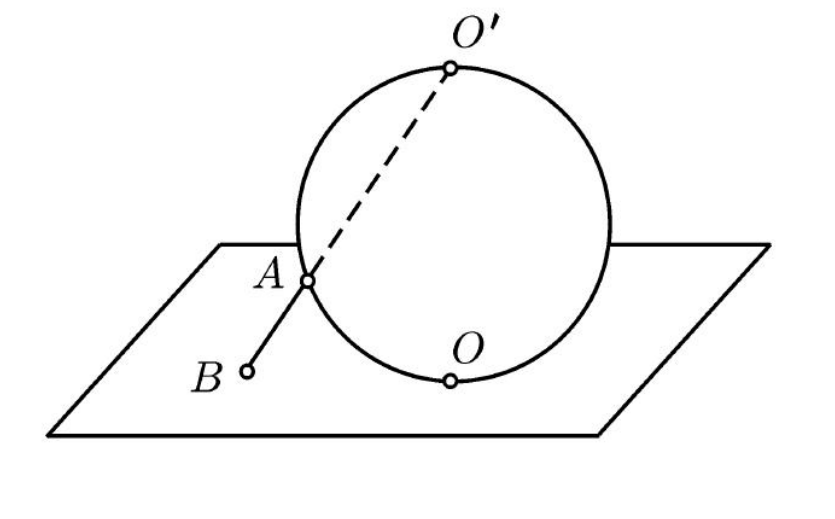
\includegraphics[width=0.5\textwidth]{par26sphere.png}
\end{center}

\subsubsection*{Двойственный граф}

\begin{defn}
    $G = (V, E, F)$ --- плоский связный мультиграф.

    Граф $G^*$, двойственный $G$: каждая грань становится вершиной, и каждое ребро исходного графа, служившее границей между двумя гранями, переходит в ребро, соединяющие соответствующие вершины.
\end{defn}

\begin{statement}
    Для всякого плоского графа $G$ граф $G^*$ тоже плоский, и $(G^*)^* = G$.
\end{statement}

\begin{notice}
    Двойственность --- соответствие между укладками, а не между графами! Для разных укладок одного и того же графа двойственные ему графы могут быть неизоморфными.
\end{notice}

\begin{center}
    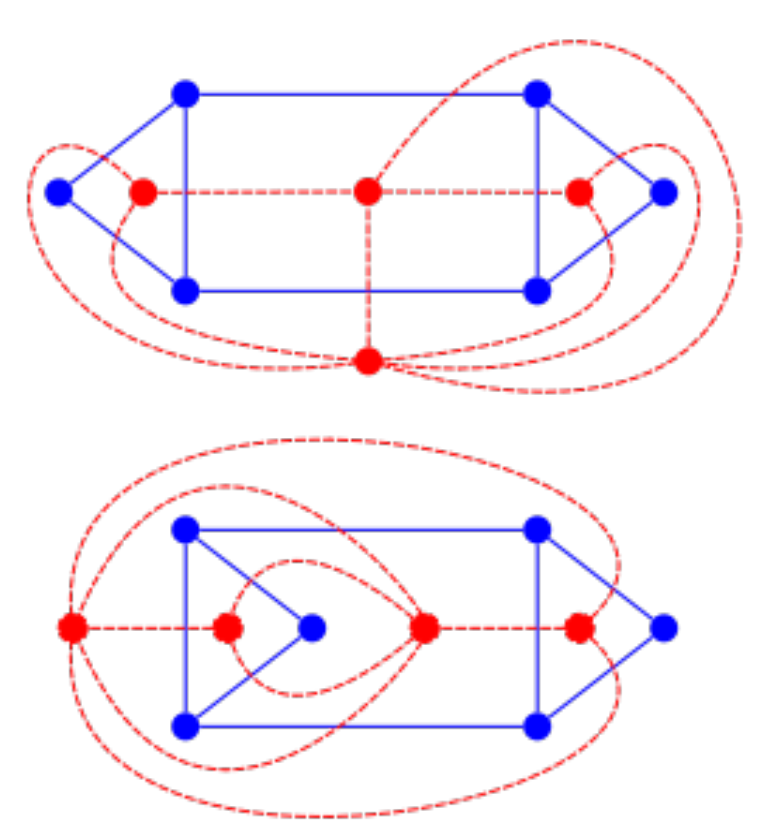
\includegraphics[width=0.3\textwidth]{par26dual.png}
\end{center}